For the final Milestone, each group member was required to individually implement different Barrelfish subsystems and then jointly integrate them at the end. This chapter delves into the \textit{shell} and was completed by \textbf{Linh}.

\subsection{Introduction}
We have a somewhat fully functioning operating system up to this point. However, to do anything with it, we'd have to shut it down, add some user code, hook that code statically into the system code, re-start the system. Then, it finally carries out whatever task we wanted to do. What if we don't want our system to run this code every time it starts? What if we simply wanted to access some resource without needing to write and compile code for it? It is also a bit silly to have to shut down the entire system in order to do any sort of dynamic task. The solution to all this is to implement a shell, which allows real-time user interaction with the system.

\subsection{Enabling User Input}
The serial device that we use to read input from a user's keyboard is the PrimeCell UART (PL011).  In Barrelfish, the driver for this runs in user-space, and is set up by mapping a frame containing the register regions into the domain where the driver will run. Although our \texttt{init} process is becoming monolithic at this point, it is still the simplest method of running this driver. So, the frame containing the register regions for the PL011 is mapped into \texttt{init} and is also where the driver runs. With this set up, processes can now access the serial driver via the RPC library to read user input or to write to the driver's output. 


\subsection{Coordinating the Shell with \texttt{init}'s Other Responsibilities}
Recall that in Milestone 6, we decided to have \texttt{init} function as all resource servers until the nameservers were implemented. At the time of implementing the shell, the nameserver functionality was not yet complete, and so \texttt{init} still must handle all RPCs. The shell must wait for user input in order to perform any operation, and this ``waiting" cannot block \texttt{init}'s other responsibilities. This is done via device interrupts and using a separate thread to handle all commands invoked through the shell. 


In Milestone 6, we had created a separate waitset for each RPC channel, and a separate thread for each of them, waiting to dispatch events. In order to not interfere with the handling of these events, the shell receives interrupts from the UART driver on its own LMP channel, in which there is a separate thread that waits on these interrupts and handles them in sequence. So, at any given time in \texttt{init}, there may be multiple threads waiting on its own waitset for either servicing an RPC call, or a user-given shell command (See Figure \ref{figure:m7-shell-threads}). It was particularly important to use device interrupts to retrieve user-input, since the shell is running in \texttt{init}. Polling the device for user-input would've been extremely wasteful usage of \texttt{init}'s resources, and would slow down RPC messaging as a whole. With this layout, the shell should never block any other activity occurring in the system.  

\begin{figure}[ht]
    \centering
    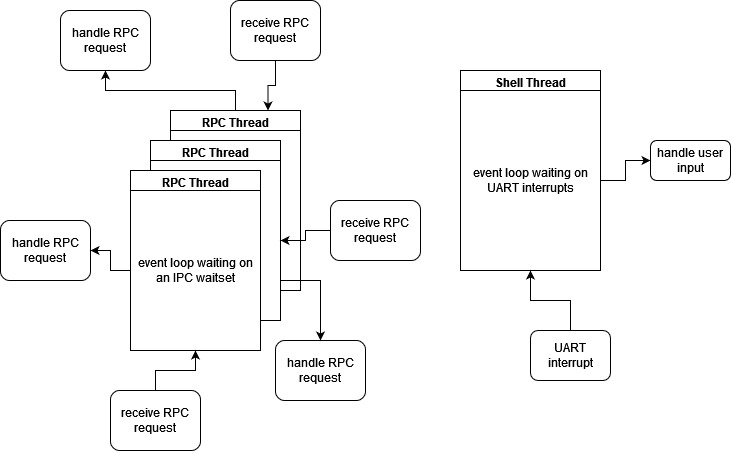
\includegraphics[width=0.8\columnwidth]{images/m7-shell-threads.jpg}
    \caption{The many threads running in \texttt{init} at any given time}
    \label{figure:m7-shell-threads}
\end{figure}

\subsection{Shell Commands}
It was pretty straightforward to implement the various commands the user can enter into the shell, since most of the functionality already existed, it just needed to be called. There is much not design required for this. The general sequence of events that occur during command execution are: 

\begin{enumerate}
    \item Receive user input
    \item Buffer the user input until a newline character is entered
    \item Upon receiving a newline, interpret the buffered input as a command (and perform the appropriate argument verification)
    \item Handle the command synchronously using pre-existing functionality by simply calling it
    \item If the command is meant to happen asynchronously, create a new thread to execute it. Store any required state upon the thread exiting.
\end{enumerate}

The full list of supported commands are:

\begin{itemize}
    \item \texttt{echo [string] ...} - prints out the given string of characters 
    \item \texttt{run\_memtest [n]} - allocates n bytes of memory, then tries to write and read them
    \item \texttt{run [cmdline] [\&]} - runs an application with the given commandline, will be in background if ``\&" is provided
    \item \texttt{oncore [coreid] [cmdline] [\&]} - same as ``run", however allows specification of which core to run on
    \item \texttt{ps} - lists out active running processes
    \item \texttt{kill [pid]} - kills the process with the given pid
    \item \texttt{help} - lists all available commands
    \item \texttt{ls} - lists the current files and directories in the current directory
    \item \texttt{mkdir [path]} - create a new directory at the given path
    \item \texttt{rmdir [path]} - removes a directory at the given path
    \item \texttt{cat [path]} - dumps the contents of the file at the given path
    \item \texttt{rm [path]} - removes the file at the given path
    \item \texttt{time [command]} - prints the time taken to execute the command in microseconds
\end{itemize}

\subsubsection{A ``Fake" Filesystem}
A core functionality to any shell is to expose the filesystem to the user. However, we unfortunately did not have a real one, and the filesystem related commands, \texttt{ls, mkdir, rmdir, cat, rm}, were implemented with the provided \texttt{RAMFS} library. The commands only work on ``temporary" files and directories, which exist only during the run-time of the system since there is no persistent file system available to save them to. In order to demonstrate the \texttt{cat} command, a temporary text file was created upon system startup simply for the purposes of calling \texttt{cat} upon it.

\subsubsection{Process Management Through the Shell}\label{m7-shell-pm}
Another core functionality of a shell is to allow the user to arbitrarily run any application they wish. Our current OS isn't quite there yet, since we don't have a filesystem. The user can run any application that has been compiled in one of the multiboot images that are ``hardcoded" into our OS.  
The \texttt{run} and \texttt{oncore} commands allow for this, and require some process management. In order to capture the exit code of a process to support the \texttt{\$?} variable, upon handling one of these commands, the shell must wait for the process to exit. Luckily, this was previously implemented in Milestone 4. However, unluckily, it was intended to be called through RPCs by processes \textit{other than} the process management server. 
%, when the user enters \texttt{run hello}, for instance, to start a process in the foreground, the shell-handling thread in \texttt{init} must wait for the \texttt{hello} process to exit. 

Due to our \texttt{init} process becoming a monolith that now includes the shell and the process manager, this required slightly adapting the process management functions to allow \texttt{init}'s shell-handling thread to wait on a process. At a high-level, this is done through waitsets, in which the shell creates a separate waitset for waiting on processes to exit. If the process is run in the foreground, waiting on this waitset is done in the same thread as the one which waits on the UART interrupts so as to allow the user-given process to ``consume" the shell console (Refer to Figure \ref{figure:m7-shell-proc-wait}). If the process is run in the background, a separate thread is created to wait on it to exit, allowing the shell-handling thread to continue to receive user input. 

\begin{figure}[ht]
    \centering
    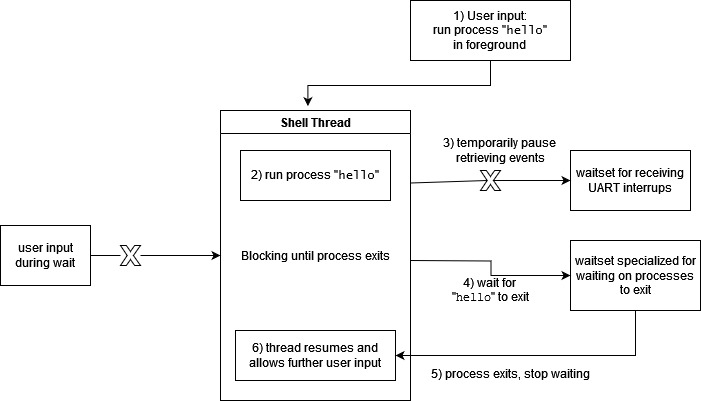
\includegraphics[width=0.8\columnwidth]{images/m7-shell-proc-wait.jpg}
    \caption{The shell thread running a foreground process}
    \label{figure:m7-shell-proc-wait}
\end{figure}

\subsection{Alternatives: Using a Separate Process for the Shell}
A more sophisticated approach to running the UART driver, and the shell, would've been to create a separate process that acted as the terminal server. The primary reasons in which this approach was not taken are:

\begin{itemize}
    \item It is much simpler to not have to set up an entirely separate process for the shell, which would require \texttt{init} to know about this server and keep track of it somewhere to allow other processes to bind to it. Furthermore, we would need to move the RPC handlers (which currently live in \texttt{init}) for writing and reading from the serial driver into this process, and ensure that it can receive requests from other processes. This is not particularly complicated, however, it does require some shifting around of code and can introduce a lot of unexpected problems that we didn't have time to deal with.
    \item In anticipation for the completed nameserver, we felt that it would be wasted effort to try to set up the terminal server in a rudimentary way before a proper nameservice binding mechanism was in place. However, since the nameserver ended up not completed, the shell ended up never migrating to its own process.
\end{itemize}

Although running the shell in \texttt{init} is easier and can work for simple use cases, it is not very good design for a system pushed out to production. The process management described in Section \ref{m7-shell-pm} highly coupled the shell's code with that of the process manager. The shell must deal with waitsets and closures, that are normally fully abstracted away from the client during an RPC. However, this coupling is inevitable due to the fact that the process manager itself is not meant to be waiting on processes to exit. To further develop the shell on top of this would definitely require de-coupling the two by moving the shell into a separate process.



